\section{IR and Collinar Divergences}
Beyond the LO (Leading order) diagrams singularities can occur. Consider first the process $ e^- e^+ \rightarrow q\bar{q}g $

\begin{figure}[ht!]
\centering
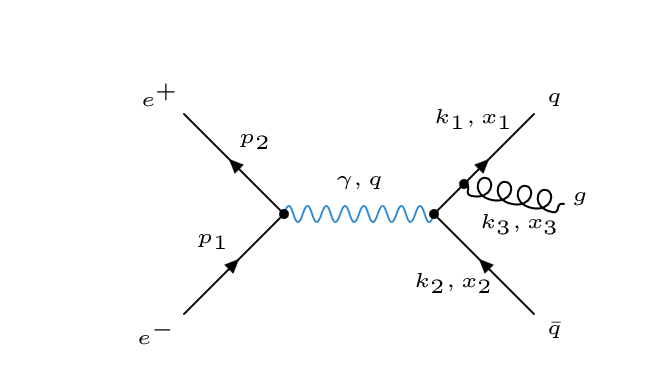
\includegraphics[width=0.85\textwidth]{images/Intro/IRCol.png}
\end{figure}

In order to calculate the cross section of this diagram, contemplate the gluon emission from the (anti)-quark. Since the calculation is quite long, concentrate on the final result:
\begin{figure}[ht!]
\centering
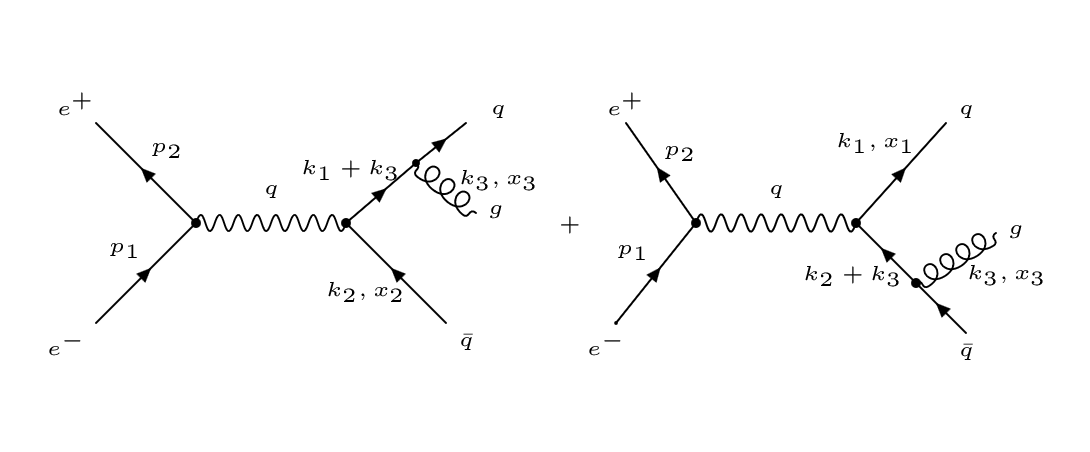
\includegraphics[width=0.85\textwidth]{images/Intro/IRColMatrix.png}
\caption{Left diagram $  e^- e^+ \rightarrow qg\bar{q} $ and right $ e^- e^+ \rightarrow q\bar{q}g $}
\end{figure}

\begin{equation}
\begin{split}
&A= \frac{\bar{u}(k_1)(-ig_s\gamma^{\nu}\times T^a)[-i(\not{k_1}+\not{k_3})](-iee_q \gamma^{\mu})v(k_2){\epsilon_{\mu}}^{\lambda_1}{\epsilon_{\nu}}^{\lambda_2*}}{(k_1 + k_3)^2}\\ 
&- \frac{\bar{u}(k_1)(-iee_q \gamma^{\mu})[i(\not{k_2}+\not{k_3})](-ig_s\gamma^{\nu}\times T^a)v(k_2){\epsilon_{\mu}}^{\lambda_1}{\epsilon_{\nu}}^{\lambda_2*}}{(k_1 + k_3)^2}\\
\Rightarrow &A=-g_s T^a[ \frac{\bar{u}\:\not{\epsilon}\:(\not{k_1}+\not{k_3})\:\Gamma \:v}{(k_1 + k_3)^2} - \frac{\bar{u}\:\Gamma\:(\not{k_2}+\not{k_3})\:\not{\epsilon} \:v}{(k_2 + k_3)^2}] \:\:\:\:\text{with} \:\:\Gamma=(-iee_q \gamma^{\mu}){\epsilon_{\mu}}^{\lambda_1}
\end{split}
\end{equation}
Under considering that the partons are on-shell, we get:
\begin{equation}
 A=-g_s T^a[ \frac{\bar{u}\:\not{\epsilon}\:(\not{k_1}+\not{k_3})\:\Gamma \:v}{2k_1 \cdot k_3} - \frac{\bar{u}\:\Gamma\:(\not{k_2}+\not{k_3})\:\not{\epsilon} \:v}{2k_2 \cdot k_3}]
\end{equation}
In the soft limit with $k_0 \rightarrow 0$ we can factorize $ A_{soft} $ the amplitude in two parts:
\begin{equation}
 A=-g_s T^a[ \frac{k_1\:{\epsilon}}{k_1 \cdot k_3} - \frac{k_2\:{\epsilon}}{k_2 \cdot k_3}] A_{born} \:\:\:\:\:\:\:\:\:\:\:\:\:\:\:\:\:\text{with}\:\: A_{born}= \bar{u}\: \Gamma \:v
\end{equation}
 Where one part contains all information about colour and momenta and the other, $ A_{born} $ involves all spin information.
If one calculates the cross section for it, one gets:
\begin{equation}
\begin{split}
A=&-C_F g_s^2 \sigma^{born} \int \frac{d^3 k}{2k_0 (2{\pi})^3} 2(\frac{k_1 \cdot k_2}{(k_1 \cdot k_3)(k_2 \cdot k_3)})\\ 
&-C_F g_s^2 \sigma^{born} \int dcos\: \theta\: \frac{d k_0}{k_0} \frac{4}{(1-cos\: \theta)(1+cos\: \theta)}
\end{split}
\end{equation}
The energy fraction is defined as:
\begin{equation}
x_i = \frac{2E_i}{\sqrt{s}}=\frac{2q\: \cdot\: k_i}{s}
\end{equation}
It can be shown that $ \sum x_i =2  $ and thus, that only two of them are independent.

The partonic differential cross section with respect to the quark and anti-quark momentum fractions is given by:
\begin{equation}
\frac{d^2 \sigma}{dx_1 dx_2}= (\frac{4\pi \alpha}{s})\sum {e_i}^2 
\frac{2\alpha_s}{3\pi} \frac{{x_1}^2+{x_2}^2}{(1-x_1)(1-x_2)}
\end{equation}

There are three singularities within the final result. 
If the emitted photon is collinear to the outgoing quark or anti-quark $ (x_1 \rightarrow 1 \:\text{or}\: x_2 \rightarrow 1) $ and when the emitted gluon is soft $ (x_1 \rightarrow 1\: \text{and}\: x_2 \rightarrow 1 )$.
The singularities come from the quark propagator in each diagram. The denominators contain terms proportional to $ \frac{1}{(k_i + k_j)^2}  $. We can eliminate the quark mass under on-shell condition so that:
\begin{equation}
\frac{1}{(k_i + k_j)^2}=\frac{1}{2k_i \cdot k_j}=\frac{1}{2E_iE_j(1-cos\theta_{ij})}=\frac{1}{s(1- x_k)}
\end{equation} 
can show all possibilities for three partons through a triangle:

\begin{figure}[h!]
\centering
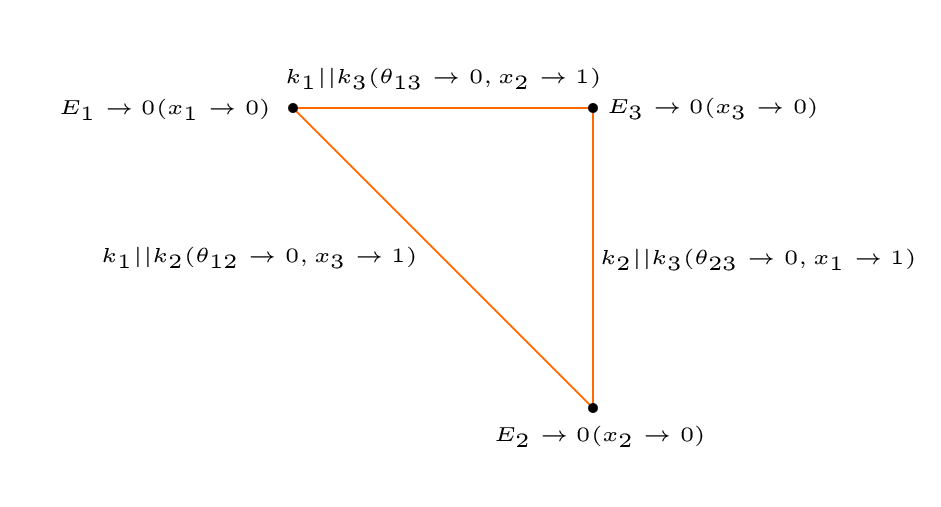
\includegraphics[width=0.85\textwidth]{images/Intro/triangle.png}
\caption{three-parton configurations at the boundaries
of phase space}
\end{figure}

According to KLN-Theorem, IR singularities must cancel when summing the transition rate over all degenerate (initial and final) states.
The sum of the integrals $ \int_R $ and $ \int_V $ over the phase space is finite. However, this is not true for the
individual contributions.
\begin{figure}[ht!]
\centering
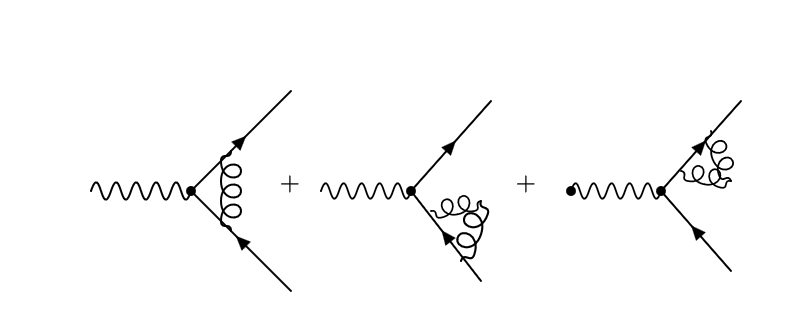
\includegraphics[width=0.85\textwidth]{images/Intro/virtual.png}
\caption{Virtual corrections: one-loop corrections to $  e^- e^+ \rightarrow q\bar{q} $}
\end{figure}
We will use deep inelastic scattering (DIS) to show how the infra-red singularities are absorbed in the parton distributions~\cite{Cunha13}.
\newpage
\section{Hard scattering}
In the last section it was seen that IR singularities occur in QCD due to the collinearity of two partons or the soften energy of one parton. These divergences occur long time after the intial hard scattering (long distance physics). Fortunately, the infrared-safe observables are calculable in perturbative QCD.  But this is not the best way to solve this problem. An interesting way for this is the factorization theorem. By this theorem the singularities of long-distance physics are removed from the partonic cross section and factorized into the parton distribution of the sleeping hadrons. This is even feasible for all orders. The background idea is that the partonic cross section is then calculable in perturbation theory. This in turn means that you can use the deep inelastic scattering and thereby absorb the infrared singularities in the parton distributions. 
Consider the hadron hadron scattering:
\begin{equation}
\sigma = \sum_{ij} \int dx_1 dx_2 f_i(x_1, \mu^2)f_j(x_2, \mu^2) \sigma_{ij}(x_1, x_2, Q^2/\mu^2... )
\end{equation}
\begin{figure}[h!]
\centering
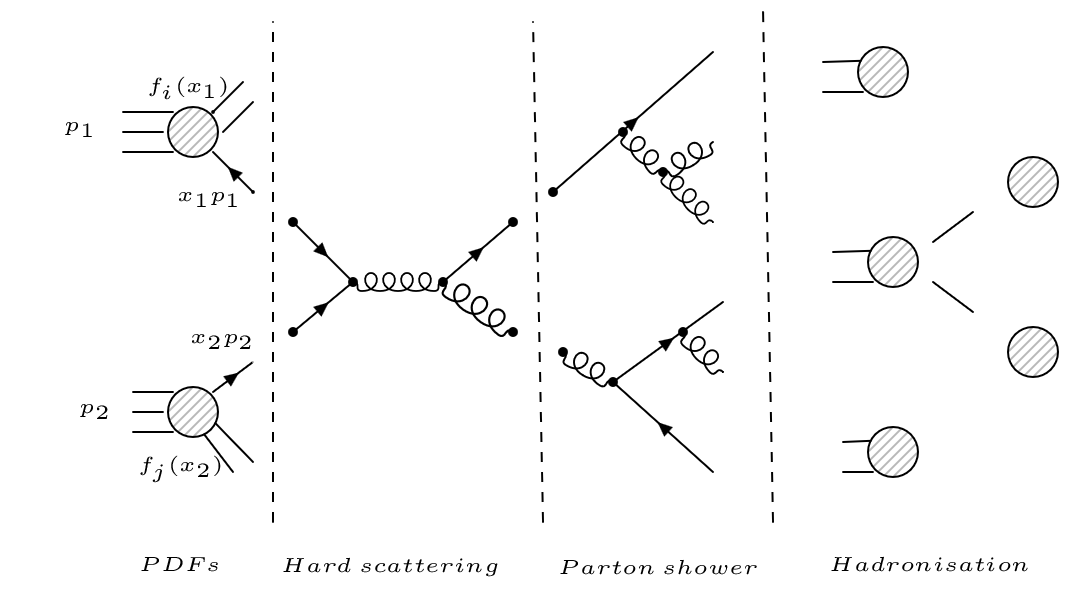
\includegraphics[width=0.85\textwidth]{images/Intro/Hard.png}
\end{figure}
With a factorisation scale $ \mu $ the long and short-distance physics could be separated. Partons with a greater momentum than $ \mu $ participate in the hard-scattering and partons with less momentum are considered as components of the hadron structure and accordingly absorbed in the parton distribution ~\cite{Nagy:2006kb}.
The DIS cross section can be written as ~\cite{Ellis:1991qj}
\begin{equation}
\frac{d^2 \sigma}{dx dQ^2}=\frac{4\pi \alpha^2}{x Q^4}[(1-y)F_2 (x, Q^2)+xy^2 F_1(x, Q^2)]
\end{equation}
In this case, the structure function need to be introduced: 

\begin{equation}
{{F}_2}^{exp} (x)= \sum_i {e_i}^2 x f_i(x)
\end{equation}

It is defined as the charge weighted sum of the parton momentum densities which describe the probability that the parton carries a momentum
fraction between $ x $ and $ \partial x $ of the proton momentum. The index $i$ denotes the quark flavour. Parton distributions are non-pertubative. fortunately it is universal and it is obtained from fit to the data for a particular factorization scheme and use them for other processes.\\
The perturbative evolution kernel of a parton
distribution due to splitting can be described by the solution of DGLAP evolution equation~\cite{Ward:1995xy}.  It is based on the collinear factorization property of QCD. Fixing the accuracy of the calculation and the factorization scheme the evolution kernel is well defined.  
\begin{equation}
\frac{\partial f(x, \mu^2) }{\partial \: ln \:\mu^2}=
\frac{\alpha_s}{2\pi}\int_{x}^{1}\frac{dy}{y} f_j(y, \mu^2) P_{ij}(\frac{x}{y})+O({\alpha_s}^2)
\end{equation}
This is a system of coupled integral or differential equations. $ P_{ij}(\frac{x}{y}) $ represents the probability, a daughter parton $ i $ with momentum fraction $ \frac{x}{y} $ is splits from a parent parton $ j $.
The above convolution in compact notation (Mellin Convolution) in the general case:
\begin{equation}
\frac{\partial f_i(x, \mu^2) }{\partial \: ln \:\mu^2}=
\sum_{j=-n_f}^{n_f} P_{ij} \otimes f_j(\mu^2)
\end{equation}

The four splitting probabilities are illustrated in the diagram \ref{splitting} and the transitions lead to a set of $ 2n_f +1 $ coupled evolution equations.
\begin{equation}
\frac{\partial }{\partial \: ln \:\mu^2} \left(\begin{array}{c}q_s\\ g\end{array}\right)=
\frac{\alpha_s}{2\pi}\begin{bmatrix}P_{qq} & 2n_fP_{qg} \\P_{gq} & P_{gg} \end{bmatrix}\otimes\left(\begin{array}{c}q_s\\ g\end{array}\right)
\end{equation}

A parton distribution changes when a different parton splits or the parton itself splits. Parton densities can not be analytically determined, but it is possible to predict how they evolve from one scale to another. PDFs are measured in one process and use them as an input for another process.


\begin{figure}[h!]
\centering
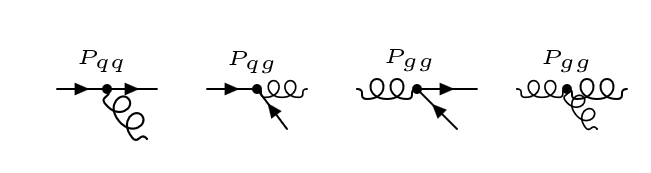
\includegraphics[width=0.85\textwidth]{images/Intro/spiliting.png}
\caption{The four splitting probabilities}
\label{splitting}
\end{figure}

\begin{equation}
	\left.\begin{aligned}
\langle\:\hat{P_{qq}}\rangle &= C_F[\frac{1+z^2}{1-z}-\varepsilon(1-z)]\\
\langle\:\hat{P_{gq}}\rangle &= T_R[1-\frac{2z(1-z)}{1-\varepsilon}]\\
\langle\:\hat{P_{qg}}\rangle &= C_F[\frac{1+(1-z)^2}{z}-\varepsilon z]\\
\langle\:\hat{P_{gg}}\rangle &= 2C_A[\frac{z}{1-z}+\frac{1-z}{z}+z(1-z)]
\end{aligned}
	\right\}
	\quad \text{Alterali-Parisi
	}
\label{Alterali-Parisi}
\end{equation}

\begin{figure}[h!]
\centering
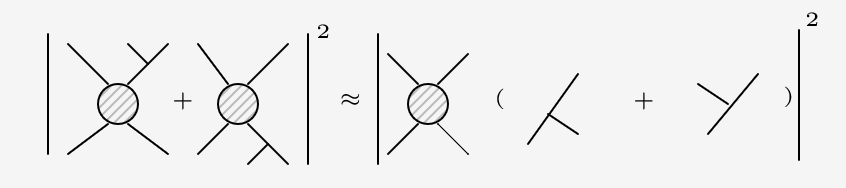
\includegraphics[width=0.85\textwidth]{images/Intro/soft.png}
\caption{Soft factorisation}
\end{figure}

\begin{figure}[h!]
\centering
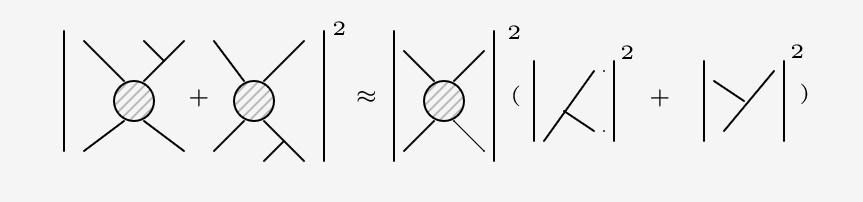
\includegraphics[width=0.85\textwidth]{images/Intro/collinear.png}
\caption{Collinear factorisation}
\end{figure}

\begin{figure}[h!]
\centering
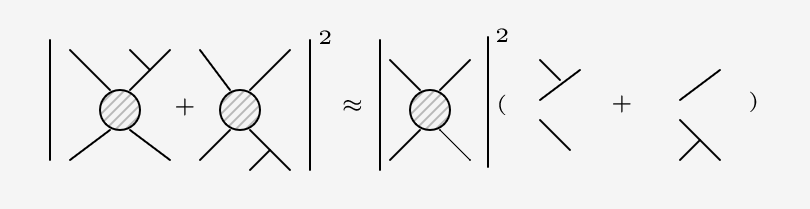
\includegraphics[width=0.85\textwidth]{images/Intro/factorization.png}
\caption{Dipole/Antenna factorisation}
\end{figure}

\section{Subtraction method}
The subtraction term is constructed as a sum over all possible dipole configurations, i.e. all possible combinations of two partons are formed to build an emitter while every single one of the remaining partons is considered a spectator.  
\begin{equation}
|A|^2 = |{A^{(0)}}_m|^2 +  |{A^{(0)}}_{m+1}|^2+ 2Re({A^{(0)*}}_{n}{A^{(1)}}_{m})
\end{equation}
Where $ |{A^{(0)}}_m|^2 $ is the tree level contribution (Born sector) from LO and has no divergences, $ |{A^{(0)}}_{m+1}|^2+ 2Re({A^{(0)*}}_{m}{A^{(1)}}_{m}) $ comes from NLO and they are each divergent. The problem in this case is the Integrals cannot be combined due to different phase space dimensions:

\begin{equation}
\sigma^{NLO} = \int_{m+1} \partial \sigma^R +\int_{m} \partial \sigma^V
\end{equation}
The real and virtual contributions are both IR divergent and need to be regularised in $ d = 4-2\epsilon $ dim.
To tackle this problem one can use the subtraction method in that way one add and subtract a local counter term $ \partial \sigma^A $ with same singularity structure as terms $ \partial \sigma^R $ to the integral. $ \partial \sigma^A $ approximates the soft and collinear singularities of $ \partial \sigma^R  $.
\begin{equation}
\sigma^{NLO} = \int_{m+1} [\partial \sigma^R -\partial \sigma^A]+\int_{m} [\partial \sigma^V+\int_1 \partial \sigma^A]
\end{equation}
In this case, we can safely set $ \epsilon \rightarrow 0 $ for $ \partial \sigma^R |_{\epsilon \rightarrow 0}  -\partial \sigma^A |_{\epsilon \rightarrow 0} $ and calculate the integral numerically in 4-dimensions. On the other side, integrate over the one-parton phase space is integrated over analytically to explicitly cancel poles and then $ \epsilon $ is set to $ 0 $.
\begin{equation}
\sigma^{NLO} = \int_{m+1} [\partial \sigma^R |_{\epsilon \rightarrow 0}  -\partial \sigma^A |_{\epsilon \rightarrow 0}]+\int_{m} [\partial \sigma^V+\int_1 \partial \sigma^A]_{\epsilon \rightarrow 0}
\end{equation}
The virtual contribution must be UV-finite:
\begin{equation}
\int_{m} \partial \sigma^V= \int_m [\int_{loop} \partial {\sigma^V}_{bare} + {\sigma^V}_{Counter\:term}]
\end{equation}
The addition of $\int_1 \partial \sigma^A$ to the $ \int_{m} \partial \sigma^V $ ensures that IR poles are cancelled.
The bare and counter contribution are separately divergent and have also different integral dimensions. One can use the same idea with the subtraction method to solve this problem~\cite{Catani:2002hc, Catani:1996vz}
\begin{equation}
\int_{m} \partial \sigma^V +\int_{loop} \partial {\sigma^L}-\int_{loop} \partial {\sigma^L}= \int_m \int_{loop}[ \partial {\sigma^V}_{bare}- \partial {\sigma^L}] + \int_m[{\sigma^V}_{Counter\:term}+ \int_{loop} \partial {\sigma^L}]
\end{equation}


\begin{equation}
\sigma^{NLO} = \int_{m+1} [\partial \sigma^R -\partial \sigma^A]+ \int_m \int_{loop}[ \partial {\sigma^V}_{bare}- \partial {\sigma^L}] + \int_m[{\sigma^V}_{Counter\:term}+ \int_{loop} \partial {\sigma^L}+\partial \sigma^A]
\end{equation}
\pagebreak
\section*{Determination of emission kernels}
Now we want to introduce the properties of the counter term $ \partial \sigma_A $. This term needs to have the same behaviour as $ \partial \sigma_R $ in d dimensions. This process and specific observable independent term has to be obtained in a way that is independent of the particular jet observable considered. It must be exactly integrable analytically over one-parton phase space in d and $ \partial \sigma_R -  \partial \sigma_A  $ has to be integrable via Monte Carlo methods. $ \partial \sigma_A $ acts as a local counter-term for $ \partial \sigma_B $
At this point, one should derive improved factorization formulae which are called dipole formulae. Note that the notation below is symbolic:
\begin{equation}
\partial \sigma_A = \sum_{dipoles} \partial \sigma_{B} \otimes \partial V_{dipoles}
\end{equation}
Where the sum is over dipoles for all $ m+1 $ configurations with consideration to a given m-parton state. $  \partial \sigma_{B}$ describes the color/spin
projection of the Born-level exclusive cross section.
The symbol $ \otimes $ describes phase space convolutions and sums over colour and spin indices. $ \partial V_{dipoles} $ will be computed and its singular properties matched to the real part. The Dipoles are universal in the sense that they do not depend on the hard scattering. This allows the use of a factorisable mapping from
the m + 1-parton phase space to an m-parton subspace. That will be clearer when the parametrisation is used in the next chapter. 
If we integrate over all $ m+1 $, we can write:
\begin{equation}
\int_{m+1}\partial \sigma_A =  \int_{m} \partial \sigma_{B} \otimes \sum_{dipoles} \int_{1}\partial V_{dipoles}
\end{equation}
This is the important result because this can now be written in terms of the known $ m $-sector from LO and the other term is a universal factor which contains all $ \epsilon $-poles.
\section*{Singularity Structure}

Before we begin with the collinear limit or soft limit respectively we are going to pull up the matrix element from LO which has this below general form:

\begin{equation}
{\mathcal{M}_m}^{c_1,...,c_m;s_1,...,s_m}(p_1,..., p_m)
\end{equation}

$ c_i $, $ s_i $ and $ p_i $ denote respectively the colour, spin indices and the momenta for each m-parton in the tree level matrix element in the final state.
A common method used in this case is to define a basis in colour+helicity space.
\begin{equation}
{\mathcal{M}_m}^{c_1,...,c_m;s_1,...,s_m}(p_1,..., p_m)\equiv(<c_i,..,c_m|\otimes <s_1,...,s_m|)|1,..,m>_m
\end{equation}
With $ <c_i,..,c_m|\otimes <s_1,...,s_m|)| $ as the basis and $ |1,..,m>_m $ as a vector in this space.
Thus, for the matrix element squared:

\begin{equation}
\begin{split}
\vert \mathcal{M}_m \vert^2=& (< c_i,..,c_m | \otimes < s_1,...,s_m|)(| c_i,..,c_m > \otimes | s_1,...,s_m >) < 1,..,m | 1,..,m > \\
&=\delta_{c_1 c_1},...\delta_{c_m c_m} \otimes \delta_{s_1 s_1},...\delta_{s_ms_m} \:_m < 1,..,m | 1,..,m > \:_m
\end{split}
\end{equation}
Define a colour-charge operator  $ {T_i} $ with the
emission of a gluon from each parton i:
\begin{equation}
\begin{split}
T_i = {T_i}^c |c>
\end{split}
\end{equation}
Its action onto the colour space is defined by:

\begin{equation}
<c_1,..,c_i,..c_m,c|T_i|b_1,..,b_i,..b_m>=\delta_{c_1b_1}...{T^c}_{c_ib_i}
...\delta_{c_mb_m}
\end{equation}

Where $ {T^c}_{c_ib_i} $ is the colour-charge matrix in the adjoint representation in the case of gluon emission or colour-charge matrix in the fundamental representation for the quark/anti-quark emission case. The following properties must be taken into account:
\begin{equation}
\begin{split}
&T_i \cdot T_j = T_j \cdot T_i \:\:\:\:\:\:\:\:\:\:\:\:\:\:\:\:\:\:\:\:\text{if}\:i\neq j,\: \text{commutative property}\\
& {T_i}^2 = C_i\:\:\:\:\:C_i = C_A \:\:\:\:\:\:\:\:\:\:\:\text{for gluon and} \: C_i = C_F\:\text{for (anti)quark}\\
&\sum_{i=1}^m T_i |1,...,m>_m =0 \:\:\:\:\:\text{for single state}
\end{split}
\end{equation}
Thus, the square of colour-correlated tree-amplitudes for the indices I, J referring either to final-state or initial-state partons will be~\cite{Catani:1996vz, Catani:2002hc}
\begin{equation}
\vert {{\mathcal{M}}^{I,J}}_{m,a...} \vert^2=\:_{m,a...} < 1,...,m;a,... |T_I \cdot T_J | 1,...,m;a,... >\:_{m,a...}
\end{equation}



\section*{Dipole factorisation}
Consider $(m+1)$-partons with the general matrix element~\cite{Seymour:1994we, Catani:2002hc}
\begin{equation}
\vert {{\mathcal{M}}}_{m+1} (Q; p_1,...,p_i,...,p_j,...,p_{m+1}) \vert^2
\end{equation}
We need to take collinear and soft limits which allow factorisation.
In the soft region the momentum $ p_j $ can be parametrised with $ p_j \rightarrow \lambda q, \lambda \rightarrow 0 $, where $ q $ is a arbitrary four vector and $ \lambda $ a scale parameter. 
The matrix element squared is characterised by $ \vert {{\mathcal{M}}} \vert^2 \sim \frac{1}{\lambda^2}$. and if $ p_i $ and $ p_j $ become collinear, we parametrise $ p_j = \frac{z}{1-z} p_i $. So the matrix element will be $ \vert {{\mathcal{M}}} \vert^2 \sim \frac{1}{p_i \cdot p_j}$.
This will be covered in more detail in the next chapter. Here is given a summery of the behaviour of the matrix elements in different regions.
Based on the Catani-Seymour method for (m + 1) parton matrix element, it's possible to factorise out parton $k$ to give $ \vert {{\mathcal{M}}}_{m}  \vert^2 $:
\begin{equation}
\vert {{\mathcal{M}}}_{m+1}  \vert^2 \rightarrow \sum \vert {{\mathcal{M}}}_{m}  \vert^2 \otimes V_{ij,k}
\Rightarrow \vert {{\mathcal{M}}}_{m+1}  \vert^2 \rightarrow \sum \vert {{\mathcal{M}}}_{m}  \vert^2 \otimes V_{ij,k}
\end{equation}

$ V_{ij,k} $ a singular factor including parton k and its interaction with partons i and j from the m parton amplitude. This situation can be represented by the diagram \ref{factorisationPic}.

\begin{figure}[h!]
\centering
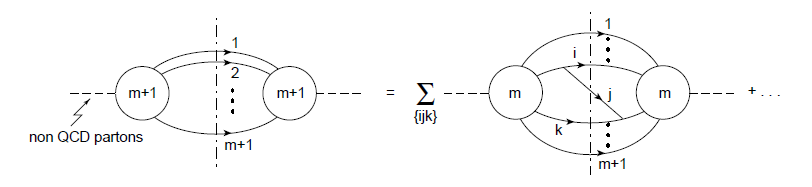
\includegraphics[width=0.85\textwidth]{images/Intro/factorisationPic.png}
\caption{Factorisation in dipole formalism}
\label{factorisationPic}
~\cite{Catani:1996vz}
\end{figure}

Here i and k are the emitters and k plays the role of a spectator. The spectator absorbs a longitudinal recoil that arises when a splitting is performedwith  all  participating  partons  remaining  on  their  mass  shells. The blobs denote the tree-level matrix elements and their complex conjugate. The dots on the right-hand side stand for non-singular terms both in the soft and collinear limits.
When the partons i and j become soft and/or collinear, the singularities are factorized into the term $ V_{ij,k} $ (the
dashed box on the right-hand side) which embodies correlations with a single additional parton k.

\begin{figure}[h!]
\centering
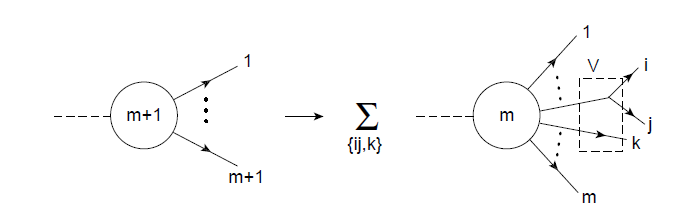
\includegraphics[width=0.85\textwidth]{images/Intro/factorisationPic2.png}
\caption{Effective diagrams for the different emitter–spectator cases.}
\label{factorisationPic2}
~\cite{Catani:2002hc}
\end{figure}

In this context the different dipole factorisation for both initial states and final states shall be presented. All these different possibilities can be seen in the diagram \ref{factorisationPic2}.
$  \mathcal{D}_{ij,k} $ describes the final state emitter and final-state spectator (FF), $  {\mathcal{D}^a}_{ij} $ the final-state emitter and initial-state spectator (FI), $ {\mathcal{D}^{ai}}_{k} $ the initial-state emitter and final-state spectator (IF) and $ \mathcal{D}^{aj,b} $ the initial-state emitter and initial-state spectator (II).
The dipole factorisation formula for all these possibilities is \cite{Schumann:2007mg}
 \begin{equation}
 |\mathcal{M}_m+1|^2 = \displaystyle\sum\limits_{i,j} \displaystyle\sum\limits_{k\neq i,j} \mathcal{D}_{ij,k} +\displaystyle\sum\limits_{i,j} \displaystyle\sum\limits_{a} {\mathcal{D}^a}_{ij}+\displaystyle\sum\limits_{a,i} \displaystyle\sum\limits_{k\neq i} {\mathcal{D}^{ai}}_{k}+\displaystyle\sum\limits_{a,i} \displaystyle\sum\limits_{b\neq a} \mathcal{D}^{aj,b}+...
 \end{equation}
In each term $ i, j $ and $ k $ denote final-state partons and a and b stand for initial-state partons. Note that there are many not-divergent contributions or diagrams, which are marked here with the dots. In this Work the first contribution final-state emitter and final-state spectator (FF) is used. Later it becomes clear how to deal with the formula.

\begin{figure}[h!]
\centering
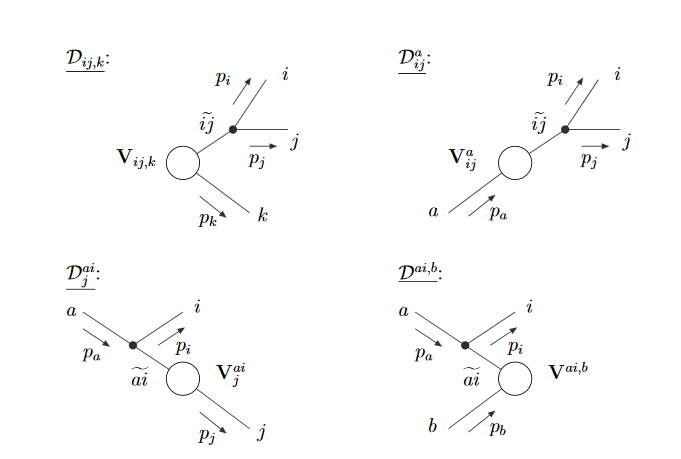
\includegraphics[width=0.85\textwidth]{images/Intro/Dipole.png}
\end{figure}

The circle in the center of each sub diagram presents the m-partons matrix element and the tilde labels the collinear splitting process for the initial or final states.
For this work, the first upper diagram with final-state singularities without initial-state partons, is completely sufficient and is discussed here in detail with its formula.
The matrix element for this is written:

\begin{equation}
\vert {{\mathcal{M}}}_{m+1}  \vert^2 = < 1,...,m+1 || 1,...,m+1 > = \sum_{k \neq i,j} {{\mathcal{D}}}_{ij,k}(p_1,...,p_{m+1}) +\text{finite terms}
\end{equation}

The first term with the sum over dipoles is divergent as $ p_i \cdot p_j \rightarrow 0 $. 
For the case of final-state emitters with a final-state spectator,for instance, the individual dipole contributions read
\begin{equation}
 {{\mathcal{D}}}_{ij,k}(p_1,...,p_{m+1}) = \frac{-1}{2p_i \cdot p_j} \:\:_m<1,...,\tilde{ij},...,k,...,m+1 |\frac{T_k \cdot T_{ij}}{{T_{ij}}^2} V_{ij,k}| 1,...,\tilde{ij},...,k,...,m+1 >\:_m
\end{equation}

Where $ T_k \cdot T_{ij} $ are the color charges of spectator and emitter

$ V_{ij,k} $ splitting kernel in helicity space of emitter
explicit form depends on parton type become proportional to Altarelli-Parisi splitting functions \ref{Alterali-Parisi} and eikonal factors
in collinear and soft limits.\\
when all the involved partons are assumed to be massless. The occurring $ m $-parton states are constructed from the original $(m+ 1)$-particle matrix element by replacing the partons $ i $ and $ j $ with the new parton $  \widetilde{ij} $ , and the original parton $ k $ with the $  \widetilde{k} $ spectator. In the massless case, their momenta are given by:
\begin{equation}
\begin{split}
&{\tilde{p}^{\mu}}_{ij} = {p_i}^{\mu}+{p_j}^{\mu}-\frac{y_{ij,k}}{1-y_{ij,k}}{p_k}^{\mu}\\
&{\tilde{p}^{\mu}}_{k} = \frac{1}{1-y_{ij,k}}{p_k}^{\mu}\\
&\text{with}\:\:\:y_{ij,k}=\frac{p_i \cdot p_j}{p_i \cdot p_j+p_j \cdot p_k+p_k \cdot p_i}
\end{split}
\end{equation}
Note, that momenta are on-shell. Due to momentum conservation ${p_i}^{\mu}+{p_j}^{\mu}+{p_k}^{\mu}= {\tilde{p}^{\mu}}_{k} +{\tilde{p}^{\mu}}_{ij} $. 


\newpage